\documentclass[aps,prb,reprint,showpacs,floatfix,superscriptaddress, onecolumn, nofootinbib, 9pt]{revtex4-2}

\usepackage{amsmath,amsthm,amssymb}
\usepackage{graphicx}% Include figure files
\usepackage{dcolumn}% Align table columns on decimal point
\usepackage{bm}% bold math
\usepackage{color}
\usepackage{epsfig}
\usepackage{multirow}
\usepackage{mathrsfs}
\usepackage{hyperref}
\usepackage{cleveref}
\usepackage{epstopdf}
\usepackage{subfigure}
\usepackage{autobreak}
\usepackage{todonotes}
\usepackage{physics}
\usepackage{bbm}



\usepackage[absolute,overlay]{textpos}

%Macros for mathematical notations

\newcommand{\V}[1]{\boldsymbol{#1}} %# vector
\newcommand{\M}[1]{\boldsymbol{#1}} %# matrix
\newcommand{\Set}[1]{\mathbb{#1}} %# set
\newcommand{\D}[1]{\Delta#1} %# \D{t} for time step size
\renewcommand{\d}[1]{\delta#1} %# \d{t} for small increment
\newcommand{\av}[1]{\left\langle #1\right\rangle } %take average

\newcommand{\sM}[1]{\M{\mathcal{#1}}} %matrix in mathcal font
\newcommand{\dprime}{\prime\prime} % double prime
%\global\long\def\i{\iota}
%\renewcommand{\i}{\iota} %i for imaginary unit
%\renewcommand{\i}{\mathsf i} %i for imaginary unit
\newcommand{\follows}{\quad\Rightarrow\quad} %=>
\newcommand{\eqd}{\overset{d}{=}} %=^d
\newcommand{\spe}[1]{\mathscr{#1}}  %important quantities in mathscr font
\newcommand{\eps}{\epsilon}

\newcommand{\response}[1]{{\color{blue}#1}} % for authors' response


\begin{document}
	\preprint{Preprint}
	
	\title{Response to Referee Comments for Manuscript BH14505}
	\author{Analabha Roy}
	\date{\today}
	
	\maketitle
	
	\vspace{1em}
	
	\noindent \textbf{Response to First Referee}
	
	\begin{enumerate}
		\item The referee says, ``\textit{A brief comparison of this work to other works on periodically driven LMG models and DMBL is needed somewhere in the introductory sections to state what is the significance and novelty of this work. }"\\
		
		\response{
			We thank the referee for this suggestion. In earlier work on periodically driven LMG models,
			the focus was on determining the onset of DMBL by looking at expectation values of local
			observable(s). Standard quantities that have been observed include magnetization, heating rate, and fidelity susceptibility. The observables were calculated by running simulations over an long duration, and localization was inferred from their dynamics over long but ultimately finite times.
			
			The novelty of our paper lies in the investigation on DMBL in the Floquet quasi-stationary states , rather than in the observable dynamics of the LMG model. Localization in the Floquet modes can be obtained from their Inverse Participation Ratios, which distinguishes between a fully localized state and a thermal state of the system. IPR ranges from scaling inversely with the Hilbert space dimension (a fully distributed or thermal state) to unity (a fully localized state). IPR calculated from Floquet modes is a better indicator of localization, as it is valid for infinite times, as opposed to observable dynamics, where very long time effects are inconclusive. We have revised and updated our introduction part to elaborate the novelty of our work.
		


}
		\item The referee says, ``\textit{On page 3, the Floquet eigenstate Thermalization hypothesis is stated without references. }".\\
		
		\response{
			We thank the referee for pointing out this mistake. In the manuscript, we have provided proper references to FETH in Page 3.
		}
		
		\item The referee says, "\textit{On page 4, after illustrating the resonances in the analytically solvable TFIM model, the authors claim, “This phenomenon is highly general and can be readily adapted to non-integrable systems”. I disagree with the statement, and clear references, if any, need to be cited to back up this statement. The manipulations made for TFIM are fine-tuned to this integrable system, and they break down the moment any integrability-breaking term is introduced. For example, if I add a longitudinal field sigma-x to the TFIM, I do not see how to adapt the procedure. }"\\
		\response{ We would like to thank the referee for this comment. We acknowledge that there may have been a lack of clarity regarding this matter in the manuscript. We have included additional content in the manuscript (one para in section 1 page 4) to elaborate on this. A detailed explanation follows:
			
		In the manuscript, we applied the RWA on the Hamiltonian following the unitary transformation to investigate localization in TFIM. Now, an additional longitudinal field $\sigma^x$ to the original TFIM Hamiltonian destroys the integrability of the model. However, this does kill the suppression of the fermion number dynamics, but not completely.  Adding a symmetry-breaking field $\sigma^x$ to the driven TFIM yields 
			\begin{equation}
				\hat{H}_{TFIM+S_x}(t) =\frac{1}{2}\left[\sum_{i} J \hat{\sigma}_{i}^{x} \hat{\sigma}_{i+1}^{x}+\sum_{i} \hat{\sigma}_{i}^{x}+h \cos (\omega t) \sum_{i} \hat{\sigma}_{i}^{z}\right]
			\end{equation}
			In order to move to the rotating frame, the transformation operator to be applied is $\displaystyle \hat{U}(t)$ is, $\hat{U}(t)=\prod_{i} \exp \left(-i \frac{h}{2 \omega} \sin (\omega t) \hat{\sigma}_{i}^{z}\right)$. The TFIM part of the Hamiltonian transforms the same way as before.	The transformation + RWA approximation for the longitudinal field works out as follows. First, we define proper angular momenta $\displaystyle S^{\mu(=x,y,z)} = \frac12\sum_i \hat{\sigma}^\mu_i$, so that we can write
			\begin{align*}
				\frac12 \sum_i \hat{\sigma}^x_i & \rightarrow\frac{1}{2} \exp \left(i \frac{h}{2 \omega} \sin (\omega t) \sum_{i} \hat{\sigma}_{i}^{z}\right)\left(\sum_{i} \hat{\sigma}_{i}^{x}\right) \exp \left(-i \frac{h}{2 \omega} \sin (\omega t) \hat{\sigma}_{i}^{z}\right) \\
				& =\left(e^{i 2 \eta S^{z}} S^{x} e^{-i 2 \eta S^{z}}\right),
			\end{align*}
			where we have used the Baker-Campbell-Hausdorff formula, together with the canonical angular momentum commutation relations. Applying the Jacobi Anger expansion again, recalling that $\eta=\frac{h}{2 \omega} \sin (\omega t)$ and taking the RWA that keeps only $n=0$'th term, yields
			\begin{equation}
				\Big(\frac12 \sum_i \hat{\sigma}^x_i\Big)^{RWA} = \left(S^{x} \cos (2 \eta)-S^{y} \sin (2 \eta)\right) \simeq \mathcal{J}_{0}\left(\frac{h}{\omega}\right) S^{x} = \mathcal{J}_{0}\left(\frac{h}{\omega}\right)\frac12\sum_i\hat{\sigma}^x_i.
			\end{equation}
		Thus, we have the full RWA for $\hat{H}_{_{TFIM+S_{x}}}(t)$,
		\begin{equation}
			\hat{H}_{_{TFIM+S_{x}}}^{R W A}= H^{RWA}+\frac12 \mathcal{J}_{0}\left(\frac{h}{\omega}\right) \sum_i\hat{\sigma}^x_i,
			\label{eq:tfim_sx1}
		\end{equation}
		where $H^{RWA}$ is the Rotated wave approximation of the regular TFIM. If drive parameters $h$ and $\omega$ are adjusted to the root of $\mathcal{J}_0\left(\frac{2h}{\omega}\right)$, then the longitudinal field survives. However, note that the Bessel function has asymptotic form $\mathcal{J}_0(x)\sim x^{-1/2}\cos(x-\pi/4)$, a good approximation for sufficiently  large $x$. In that limit, if $x$ is chosen to lie at a root, then $x\approx (2n+1/2)\pi/2$, in which case $\mathcal{J}_0(2x) \sim -x^{-1/2}/2$, which is small for sufficiently large $x$. Thus, the $\tau_x-$term in $H^{RWA}$ is very small if $h\gg\omega$, $\mathcal{J}_0\left(\frac{h}{\omega}\right)=0$, partially recovering dynamical freezing for short times at a different point.}

		\item The referee says,``\textit{In the discussion of phase crossover from thermal to DMBL, increasing N in Fig 8 appears to push the regime of the local phase to a larger drive frequency. This seems to raise the same concerns associated with the stability of disorder-induced localization, as in whether one needs infinite disorder or infinite driving frequency to
			get a localization in the thermodynamic limit. Is this the case? }".
		
		\response{    	
			We thank the referee for the comment. We have extended our simulations for larger system sizes and have verified that this is, indeed, the case. Increasing $N$ pushes the crossover point further to larger values of $\omega$, thus requiring infinite frequency at infinite size. We have updated the corresponding Fig.8 with a revised version, and have reported this in section 4 par 2.
		}
		\item The referee says,``\textit{Is the heating suppressed at points where the frequency meets the resonance condition? }".
		
		\response{
		While the concept of 'heating' is inapplicable in the integrable TFIM case (as the system never thermalizes), the heating is, indeed, suppressed at the resonance condition for the long-range LMG model, provided the frequency is large enough to take the system out of the low-frequency regime. This can be seen in the plots of standard deviation of the heating rate in figure 9 of the manuscript. There, the system is always kept at the resonance condition, but the deviation corresponds to the infinite temperature value for small frequencies, but increases as we traverse the crossover to the DMBL phase. The higher values arise due to integrable dynamics, and heating is suppressed since the IPR of the Floquet states is unity in that regime.}
		
		\item The referee says, ``\textit{The discussion related to Fig. 9 could be improved, and it is not clear to me why the standard deviation of temporal fluctuations should vanish for thermalizing systems. }"\\
		
		\response{ We thank the referee to point out the issue. We agree to improve the discussion and rectify our results. We have revised the discussion in Section IV, 3 para, as well as improved the corresponding Fig.(9) also.
			
			
			The Hamiltonian for LMG model,
			\begin{equation}
				\mathcal{H} = \frac{J}{2(N-1)}\sum_{i\neq j}\hat{\sigma}^z_i \hat{\sigma}^z_j + (h_0 +h_1 \cos(\omega t) \sum_i \hat{\sigma}^x_i
			\end{equation}
			In the full Hilbert space, considering the dc part ($h_0$) of the drive is very negligibly small, the time average of the Hamiltonian,
			\begin{equation*}
				\bar{H}_0 = \frac{J}{2(N-1)}\sum_{i\neq j}\hat{\sigma}^z_i \hat{\sigma}^z_j.
			\end{equation*}
			Similarly,
			\begin{equation}
				\left(\bar{H_0}\right)^2 = \frac{J^2}{4(N-1)^2}\sum_{i\neq j, k \neq l} \hat{\sigma}^z_i \hat{\sigma}^z_j \hat{\sigma}^z_k \hat{\sigma}^z_l
			\end{equation}
			
			The thermal variance at $T= \infty$ is given by $\displaystyle \sigma^2_{\infty} = \frac{\Tr[H^2_0]}{2^N}$. 
			
			\begin{figure}[h!]
				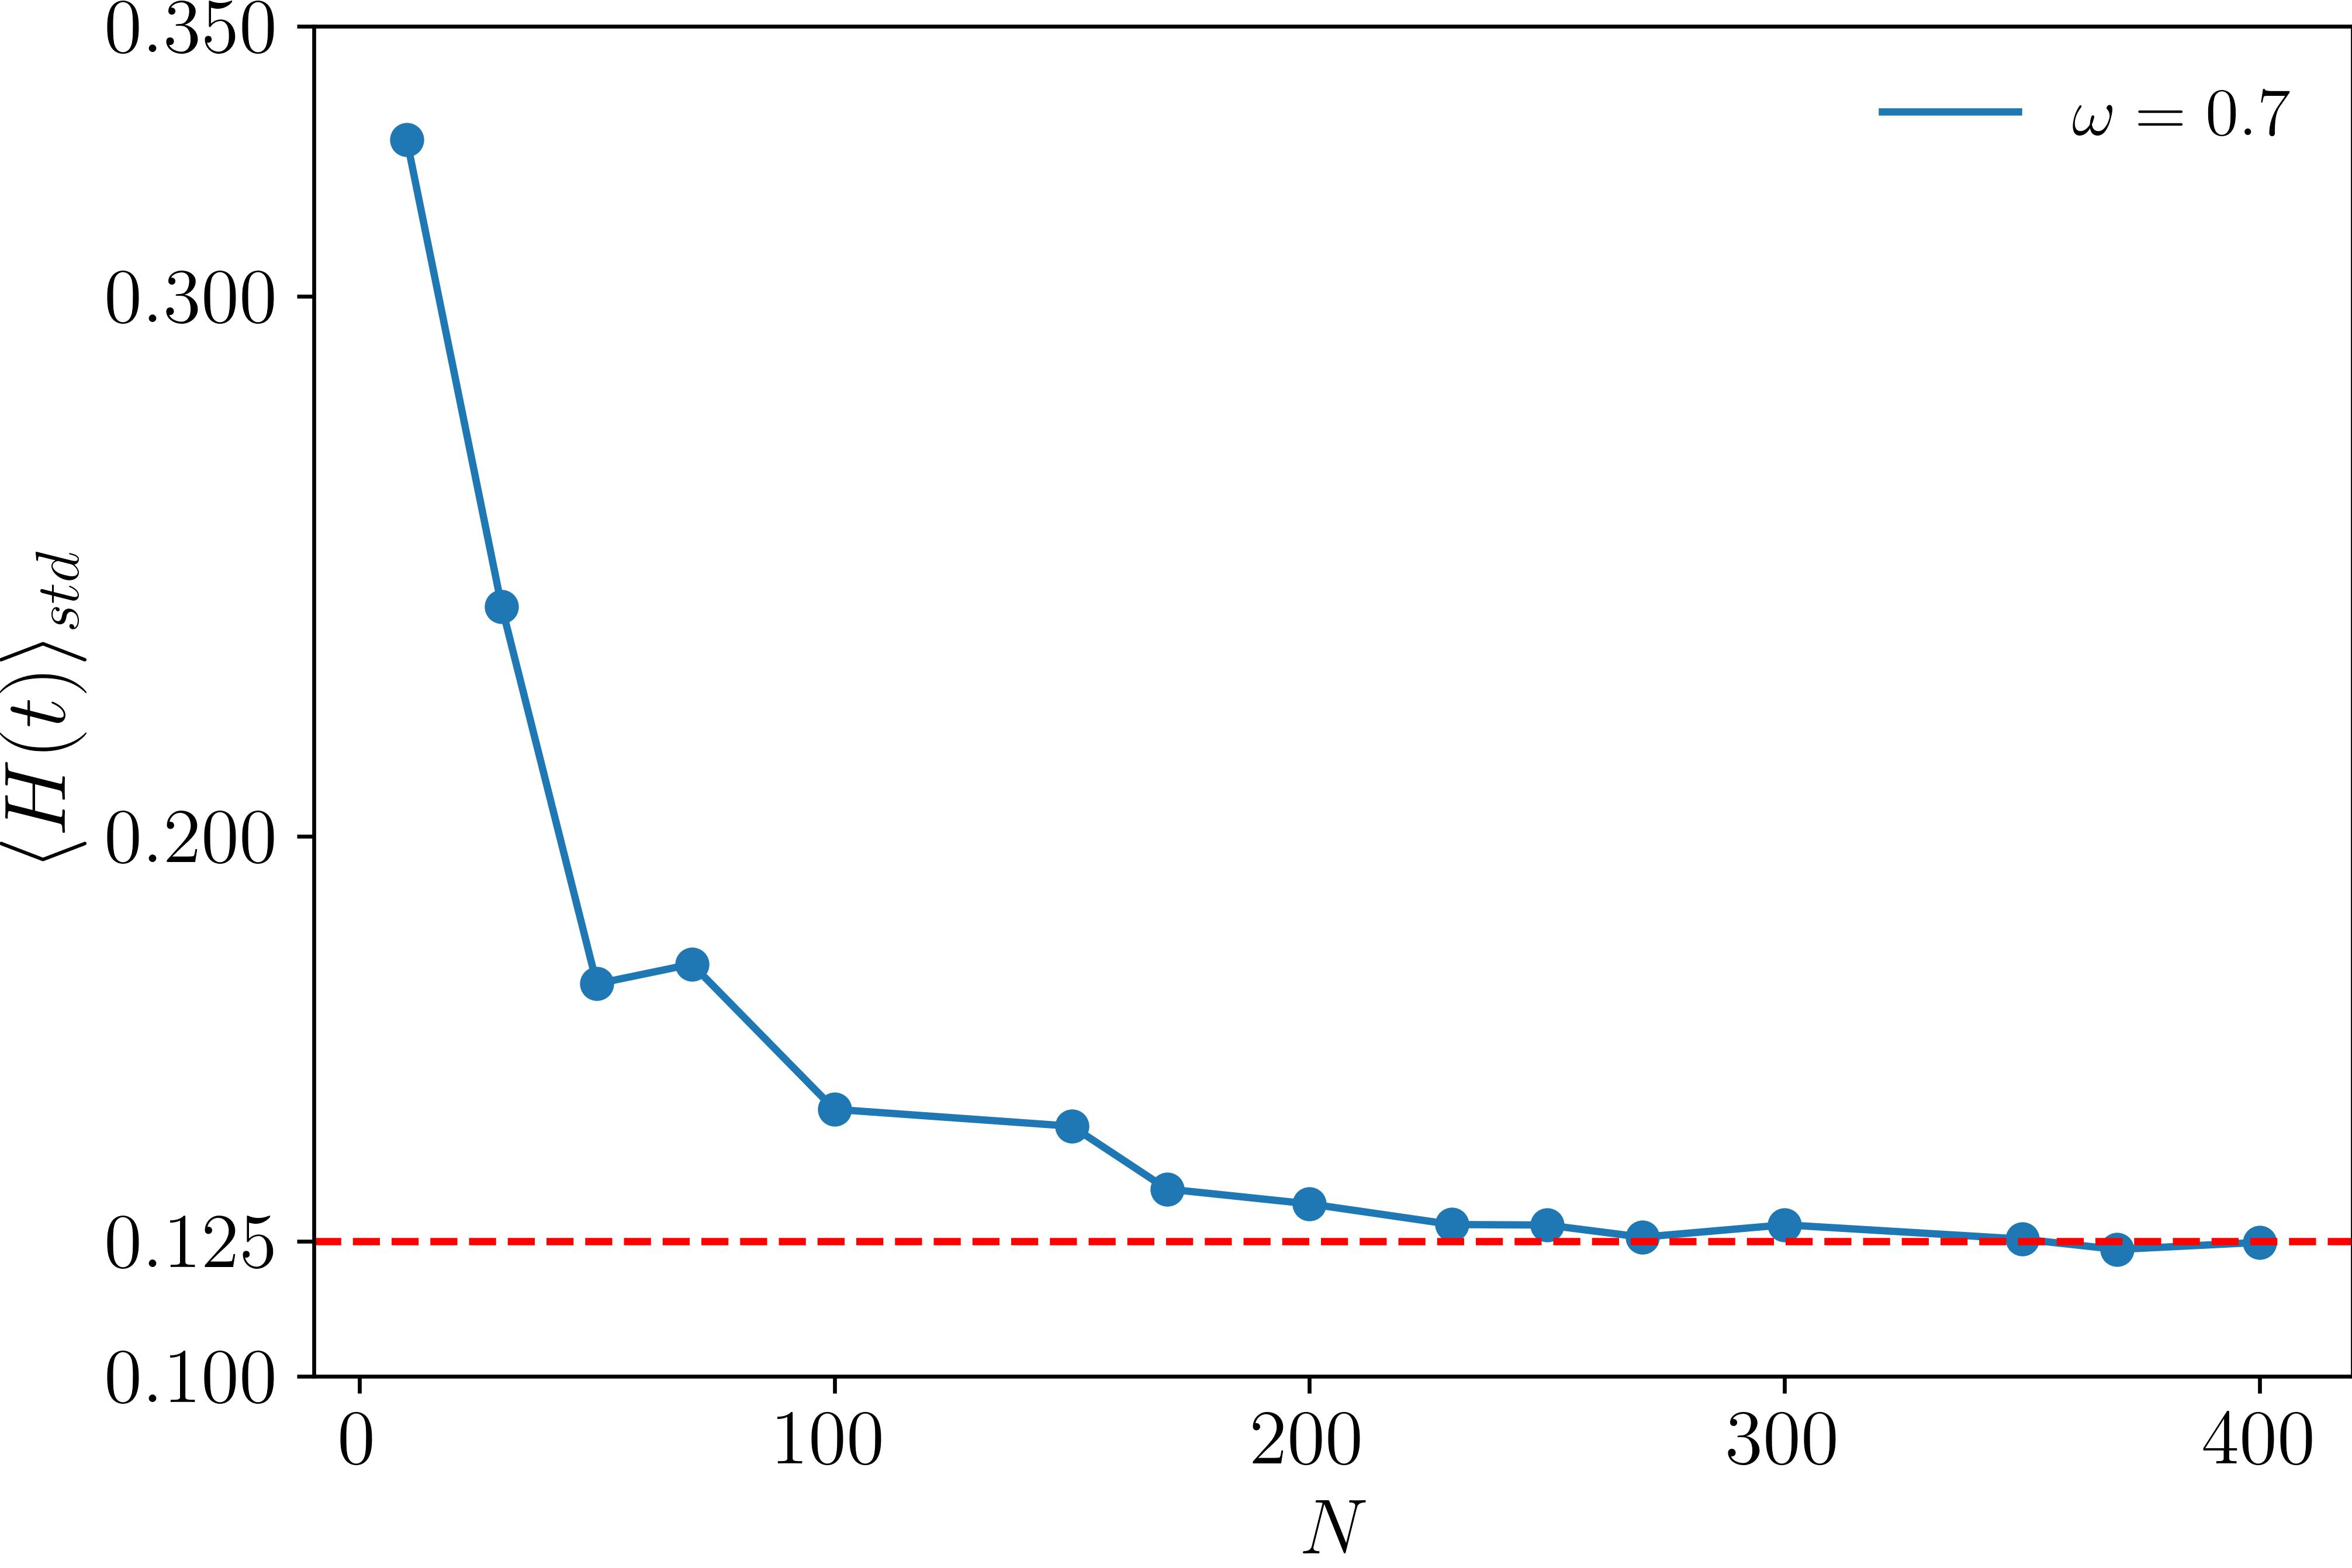
\includegraphics[width=8.5cm]{hbar_avg_std_w0.7.jpg}
				\caption{Variation of $\expval{H(t)}_{std}$ with system size(N) at small frequency $\omega=0.7$. $\expval{H(t)}_{std}$ is found to decrease as N increases and at thermodynamic limit it reaches 0.125.}
				\label{fig:std_Ns}
			\end{figure}
			
			Since $\bar{H_0}$ is traceless, and the trace part of $\left(\bar{H_0}^2\right)$, when $i,j$ and $l,k$ terms are equal, we get ,
			\begin{align*}
				\sigma_\infty^2 =& \frac{J^2}{4(N-1)^2 2^N}\Tr[\sum_{i\neq j, k \neq l} \hat{\sigma}^z_i \dots\otimes \mathbbm{1} \otimes \dots \hat{\sigma}^z_j \dots\otimes \mathbbm{1} \otimes \dots \hat{\sigma}^z_k\dots\otimes \mathbbm{1} \otimes \dots \hat{\sigma}^z_l ]\\
				=& \frac{J^2}{4(N-1)^2 2^N}   2^N \sum_{i\neq j} 1\\
				=& \frac{J^2}{4(N-1)^2} \frac{N(N+1)}{2}\\
				=& \frac{J^2}{8} \frac{N^2+N}{N^2-2N+1}.
			\end{align*}
			When $N\rightarrow \infty$,
			\begin{equation}
				\sigma_\infty^2 \simeq \frac{J^2}{8}
				\label{eq:std_inf}
			\end{equation} 
			
			For convenience, we had set $J=1$ in the manuscript. Thus, $\sigma_\infty^2 = 0.125$. The numerical result in Fig.\ref{fig:std_Ns} supports analytical results in Eq. \eqref{eq:std_inf}. Thus at low frequency $\expval{H(t)}_{std}$ goes thermal value. We have updated the manuscript with sa brief footnote summarizing this point, and added fig~\ref{fig:std_Ns} as an inset.
		}
		
		
		\vskip 2cm
		\item The referee says,``\textit{In the conclusion, it is useful to comment on whether this method could be adapted (related to my point 2) to other generic models (say
			XXZ models). }"\\
		
		\response{
		We thank the referee for the comment. We have discussed on this issue in Conclusion Sectino as well as in the Background section also.
		We would like to discuss on this matter below, 

		The generic Heisenberg model
			\begin{equation*}
				H = \frac12 \left( \sum_{i=1} J^x \hat{\sigma}^x_i \hat{\sigma}^x_{i+1} +J^y  \hat{\sigma}^y_i \hat{\sigma}^y_{i+1} + J^z  \hat{\sigma}^z_i \hat{\sigma}^z_{i+1} + h  \hat{\sigma}^z_i\right).
			\end{equation*}
			If $J^x= J^y \neq J^z=\Delta$, then it is called a XXZ model.
			
			The unitary evolution operator $\displaystyle \hat{U}(t)$ is, $\hat{U}(t)=\prod_{i} \exp \left(-i \frac{h}{2 \omega} \sin (\omega t) \hat{\sigma}_{i}^{z}\right)$. Now the Hamiltonian in rotating frame,
			
			\begin{align}
				\tilde{H}(t)_{_{XXZ}}= & \frac{1}{2} \exp \left(i \frac{h}{2 \omega} \sin (\omega t) \sum_{i} \hat{\sigma}_{i}^{z}\right)\left(\sum_{i} J \hat{\sigma}^x_i \hat{\sigma}^x_{i+1} + J \hat{\sigma}^y_i \hat{\sigma}^y_{i+1}+ \Delta  \hat{\sigma}^z_i \hat{\sigma}^z_{i+1}\right) \exp \left(-i \frac{h}{2 \omega} \sin (\omega t)\right)\nonumber\\
				= \frac12 \Bigg[& \underbrace{\exp \left(i \frac{h}{2 \omega} \sin (\omega t) \sum_{i} \hat{\sigma}_{i}^{z}\right)\left(\sum_{i} J \hat{\sigma}_{i}^{x} \hat{\sigma}_{i+1}^{x}\right) \exp \left(-i \frac{h}{2 \omega} \sin (\omega t) \sum_i\hat{\sigma}_{i}^{z}\right)}_{\mathrm{A}} \nonumber\\
				& +\underbrace{\exp \left(i \frac{h}{2 \omega} \sin (\omega t) \sum_{i} \hat{\sigma}_{i}^{z}\right)\left(\sum_{i} J \hat{\sigma}_{i}^{y} \hat{\sigma}_{i+1}^{y}\right) \exp \left(-i \frac{h}{2 \omega} \sin (\omega t) \sum_i\hat{\sigma}_{i}^{z}\right)}_{\mathrm{B}} \nonumber\\
				& +\underbrace{\Delta \left(\sum_{i}  \hat{\sigma}_{i}^{z} \hat{\sigma}_{i+1}^{z}\right)}_{\mathrm{C}}\Bigg]
				\label{eq:xxz1}
			\end{align}
		
		Utilizing angular momenta $\displaystyle S^{\mu(=x,y,z)} = \frac12\sum_i \hat{\sigma}^\mu_i$, 
		\begin{align}
		\tilde{H}_{_{XXZ}} &= 2\Bigg[\Big(S^x_i S^x_{i+1}\cos^2(2\eta) + S^y_i S^y_{i+1}\sin^2(2\eta)\Big) + \Big(S^y_i S^y_{i+1}\cos^2(2\eta) + S^x_i S^x_{i+1}\sin^2(2\eta)\Big) + \frac{\Delta}{4}\hat{\sigma}_{i}^{z} \hat{\sigma}_{i+1}^{z}\Bigg] \nonumber\\
		&= 2\Bigg[\Big(S^x_i S^x_{i+1} + + S^y_i S^y_{i+1}\Big)\cos^2(2\eta) + \Big(S^x_i S^x_{i+1} + + S^y_i S^y_{i+1}\Big)\sin^2(2\eta) + \frac{\Delta}{4}\hat{\sigma}_{i}^{z} \hat{\sigma}_{i+1}^{z}\Bigg]\nonumber\\
		&= 2\Bigg[\Big(S^x_i S^x_{i+1} + S^y_i S^y_{i+1}\Big)\big(1+\cos(4\eta)\big) + \Big(S^x_i S^x_{i+1} + S^y_i S^y_{i+1}\Big)\big(1-\cos(4\eta)\big) + \frac{\Delta}{4}\hat{\sigma}_{i}^{z} \hat{\sigma}_{i+1}^{z}\Bigg]\nonumber\\
		&= 4\Big(S^x_i S^x_{i+1} + S^y_i S^y_{i+1}\Big) + \frac{\Delta}{2}\hat{\sigma}_{i}^{z} \hat{\sigma}_{i+1}^{z}
		\end{align}
		
		}
	\end{enumerate}
	\vskip 1cm 
	\noindent \textbf{Summary of important changes to the  manuscript}
	
	
	\begin{enumerate}
		\item We have improved the discussion on how FETH can be applied at some of the non-integrable system in page(4), and discussed it with an example where a integrable breaking term such as $\hat{\sigma^x}$ is augmented to TFIM.
		\item We have improved Fig. 8 $\&$ 9.
		\item We have discussed the standard deviation of heating rate at very small drive frequency at thermodynamic limit where the numerical result corroborates the analytical result.
		\item We have briefly discussed in conclusion section, if our method of achieving a phase cross over is not possible like XXZ model. 
	\end{enumerate}
	
	\bibliography{dmbl_refs}
	
	
\end{document}